\documentclass{beamer}

\usepackage[utf8]{inputenc}
\usepackage{animate}
\usepackage{url}
\usepackage{graphicx}
\usepackage{color}
%\usepackage{listings}
%\usepackage{pythonhighlight}
%\usepackage{listings}
\usepackage{minted}
%\usemintedstyle{borland}


% Add logo in header
\usepackage{textpos}
\addtobeamertemplate{frametitle}{}{%
  \begin{textblock*}{100mm}(\textwidth-1cm,-1cm)
    
\includegraphics[height=1cm,width=1cm]{media/logo_cnr_engineering_ori.png}
  \end{textblock*}
}

\usetheme{CambridgeUS}
%\usetheme{Montpellier}
%\usetheme{Boadilla}
\usecolortheme{beaver}

\setbeamercolor{block title}{fg=gray!15!white,bg=darkred!80!black}

%% \setbeamertemplate{itemize subitem}{\color{orange}$\blacktriangleright$}
\setbeamercolor{item projected}{fg=white,bg=red}

%% \setbeamercolor{block body title text}{fg=green}
%% \usepackage{color}
%% \newcommand*{\bluebullet}{\textcolor{blue}{\textbullet}}
%% \definecolor{trueblue}{RGB}{0, 115, 197}
%% \setbeamercolor{itemize item}{fg=trueblue}


\title[PyTelTools]{PyTelTools: Python scripts and GUI to automate Telemac post-processing tasks}
\author{Luc \textsc{Duron}, Yishu \textsc{Wang}}
\institute[CNR]{Compagnie Nationale du Rhône (CNR)}
\date[XXIV\textsuperscript{th} TUC - Oct. 2017]{
  {\tiny XXIV\textsuperscript{th} \textsc{TELEMAC-MASCARET} User Conference\\
    Graz, Austria, 17-20 October, 2017}
}

% Add logo on first page
\titlegraphic{
  \hspace*{1.5cm}
  
\includegraphics[height=1.7cm]{media/logo_cnr_engineering_ori.png}
  \hspace*{2.5cm}
  
\includegraphics[height=1.7cm]{media/PyTelTools_with_text.png}
}

% Remove some navigation links
\setbeamertemplate{navigation symbols}{
  % \insertslidenavigationsymbol
  % \insertframenavigationsymbol
  % \insertsubsectionnavigationsymbol
  % \insertsectionnavigationsymbol
  % \insertdocnavigationsymbol
  % \insertbackfindforwardnavigationsymbol
}

% Affiche les numéros des références plutôt qu'une image
%\setbeamertemplate{bibliography item}{\insertbiblabel}


\begin{document}

\begin{frame}
  \titlepage
\end{frame}


\begin{frame}{Table of Contents}
  \tableofcontents
\end{frame}


\section{Context}

%\subsection{Context of the projet}

\begin{frame}{Project initiation}

  \begin{block}{Compagnie Nationale du Rhône (CNR)}
    \begin{itemize}
      \item 1\textsuperscript{st} producer of exclusively renewable energy in France
      \item 18 hydroelectric facilities on the Rhône River (3000 MW)
      \item CNR Engineering Departement (for CNR and third party)
    \end{itemize}
  \end{block}

  \pause

  \begin{block}{Needs and purpose}
    \begin{itemize}
      \item Develop non-existing features, customize it for modeller needs
      \item Automate and chain Telemac post-processing tasks
      \item Do not substitute for common post-processing graphical softwares
    \end{itemize}
  \end{block}

\end{frame}

\begin{frame}{Python Telemac Tools}


\begin{columns}[onlytextwidth]
  \begin{column}{0.4\textwidth}

    \begin{block}{Developement Guidelines}<1->
      \begin{itemize}
        \item extensible
        \item customizable
        \item accessible, easy to use
        \item robustness
        \item open-source
      \end{itemize}
    \end{block}
    \includegraphics<1>[width=0.95\textwidth]{schemas/PyTelTools_organization_empty.pdf}
    \includegraphics<2->[width=0.95\textwidth]{schemas/PyTelTools_organization.pdf}
  \end{column}

  \begin{column}{0.55\textwidth}

    \begin{block}<2->{Implementation overview}
      \begin{itemize}
        \item \textbf{core}
          \begin{itemize}
            \item parsers, base classes, ...
            \item mathematical and spatial calculations
          \end{itemize}
        \item Command Line Interface (\textbf{CLI})
          \begin{itemize}
            \item multiple arguments
            \item easily adapted, snippets (being implemented)
          \end{itemize}
        \item Graphical User Interface (\textbf{GUI})
          \begin{itemize}
            \item classic interface
            \item \textbf{Workflow} : automate, chain and monitor tasks
          \end{itemize}
      \end{itemize}
    \end{block}

  \end{column}
\end{columns}

\end{frame}

%% \begin{columns}[onlytextwidth]
%%   \begin{column}{0.65\textwidth}
%%     \begin{block}{Commande Line Interface (cli)}
%%       \begin{itemize}
%%         \item a
%%         \item b
%%       \end{itemize}
%%     \end{block}
%%   \end{column}
%%   \begin{column}{0.3\textwidth}
%%     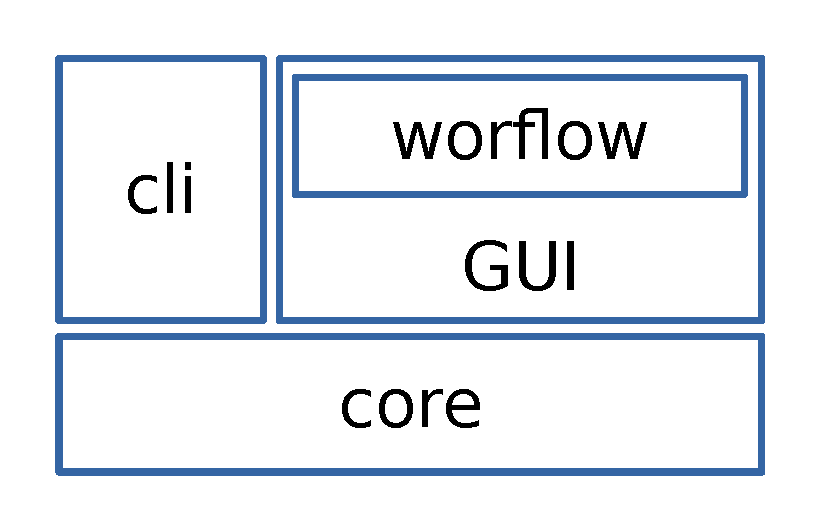
\includegraphics[width=0.95\textwidth]{schemas/PyTelTools_organization.pdf}
%%   \end{column}
%% \end{columns}


\begin{frame}{Documentation and installation}

  \begin{block}{Installation}
    \begin{itemize}
      \item Prerequisites: Python3
      \item Packages: see \href{https://github.com/CNR-Engineering/PyTelTools/blob/master/requirements.txt}{requirements.txt}  (numpy, matplotlib, PyQt5, ...)
      \item Installation procedure:
    \end{itemize}

    \inputminted[fontsize=\tiny,xleftmargin=1.5cm]{bash}{installation.sh}

  \end{block}

  \begin{block}{Documentations}
    \begin{itemize}
      \item User: \url{https://github.com/CNR-Engineering/PyTelTools/wiki}
      \item Developper: \url{https://cnr-engineering.github.io/PyTelTools}
    \end{itemize}
  \end{block}

\end{frame}


%% \begin{python}
%% import numpy as np

%% def incmatrix(genl1,genl2):
%%     m = len(genl1)
%%     n = len(genl2)
%%     M = None #to become the incidence matrix
%%     VT = np.zeros((n*m,1), int)  #dummy variable
%% \end{python}
  %\begin{lstlisting}

%% \begin{lstlisting}[language=html]

%% \begin{minted}[mathescape,
%%                linenos,
%%                numbersep=5pt,
%%                gobble=2,
%%                frame=lines,
%%                framesep=2mm]{python}
%% import numpy as np

%% def incmatrix(genl1,genl2):
%%     m = len(genl1)
%%     n = len(genl2)
%%     M = None #to become the incidence matrix
%%     VT = np.zeros((n*m,1), int)  #dummy variable
%% \end{minted}

%% \begin{lstlisting}
%% Put your code here.
%% \end{lstlisting}

%\lstinputlisting[language=Python]{filename.py}

% https://tex.stackexchange.com/questions/53998/beamer-how-text-wrapping-around-a-graphic-right-aligned
%% \begin{frame}{Folientitel}

%% \begin{minipage}[0.2\textheight]{\textwidth}
%% \begin{columns}[T]
%% \begin{column}{0.8\textwidth}
%% \begin{itemize}
%% \item Punkt 1 = text blah blah foo bar, text blah blah foo bar, text blah blah foo bar
%% \item Punkt 2= text blah blah foo bar, text blah blah foo bar, text blah blah foo bar
%% \item Punkt 3= text blah blah foo bar, text blah blah foo bar, text blah blah foo bar
%% \end{itemize}
%% \end{column}
%% \begin{column}{0.2\textwidth}
%% 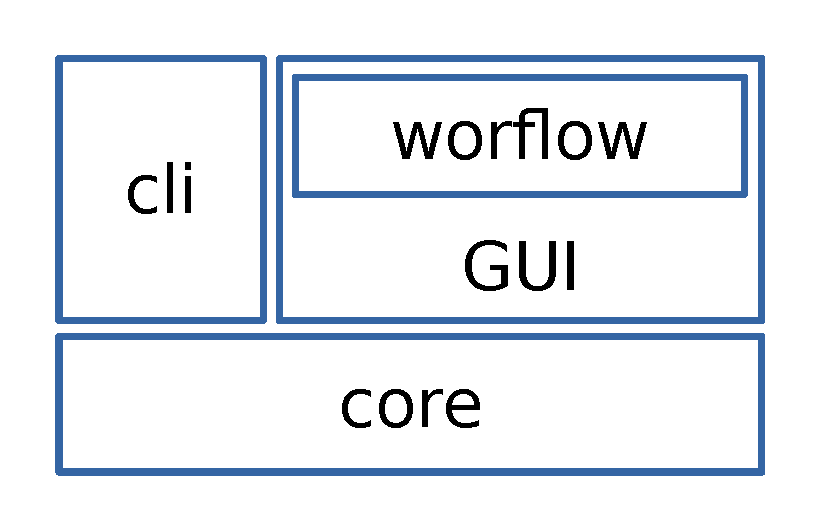
\includegraphics[width=2.5cm]{schemas/PyTelTools_organization.pdf}
%% \end{column}
%% \end{columns}
%% \end{minipage}

%% \begin{itemize}
%% \item Punkt 1 = text blah blah foo bar, text blah blah foo bar, text blah blah foo bar
%% \item Punkt 2= text blah blah foo bar, text blah blah foo bar, text blah blah foo bar
%% \item Punkt 3= text blah blah foo bar, text blah blah foo bar, text blah blah foo bar
%% \end{itemize}
%% \end{frame}



\section{Post-processing tasks}

\subsection{Categorization}

\begin{frame}{Classification of post-processing tasks}

\begin{columns}[onlytextwidth]
  \begin{column}{0.5\textwidth}

    \begin{itemize}[<+->]
      \item File conversions (shp, vtk, ...)
      \item Compute variables
      \item Mesh transformation
      \item Visualization (temporal, longitunal, cross-section, ...)
      \item Temporal analysis
      \item Vertical aggregation: depth-averaging, specific layer selection
      \item Interpolate on points, along lines (and project)
      \item Compute volume, flux
      \item Others: comparison criteria (MAD, BSS, ...)
    \end{itemize}

  \end{column}

  \begin{column}{0.45\textwidth}\centering
    %\begin{center}
      \includegraphics<2>[height=1.8cm]{media/input_variables.png}
      \includegraphics<2>[height=3.2cm]{media/exported_variables.png}
    %\end{center}

    \includegraphics<4>[width=0.95\textwidth]{media/workflow_vertical_cross_section.png}

    \includegraphics<7>[width=0.95\textwidth]{media/magland_rotated.png}
    \includegraphics<7>[width=0.95\textwidth]{media/magland_Plong.png}

    \includegraphics<8>[width=0.95\textwidth]{media/Compute_volume_Bb.png}

  \end{column}

\end{columns}
\end{frame}


%% \subsection{Some post-processing tasks}

%% \begin{frame}{A}
%%   \begin{itemize}
%%     \item A
%%   \end{itemize}
%% \end{frame}



\section{Workflow}

\subsection{Principle and notions}

\begin{frame}{Philosophy and practice}

  \begin{block}{Applications}
    \begin{itemize}
      \item sensitivity analysis, calibration processes, ...
      \item write similar post-processing files (slf, CSV)
      \item export plots, produce maps in mass
    \end{itemize}
  \end{block}
  \pause

  \begin{block}{Main workflow features}
    \begin{itemize}
      \item easy-to-use graphical interface to build pipelines
      \item visualize progress in real time
      \item ability to re-use and share pipelines
    \end{itemize}
  \end{block}
  \pause

  \begin{block}{Two levels of automation}
    \begin{itemize}
      \item \textbf{Mono}: configure and chain tasks to be run on a single simulation
      \item \textbf{Multi}: run over a set of simulations
    \end{itemize}
  \end{block}
\end{frame}


\begin{frame}{Conceptual model}
  %% \begin{itemize}
  %%   \item Directed Acyclic Graph (DAG)
  %%   \item state, options, input/output
  %%   \item reproductability (project file), commutativity, reentrancy (intermediate files)
  %%   \item FAIRE UN SCHÉMA............................
  %% \end{itemize}
  %% 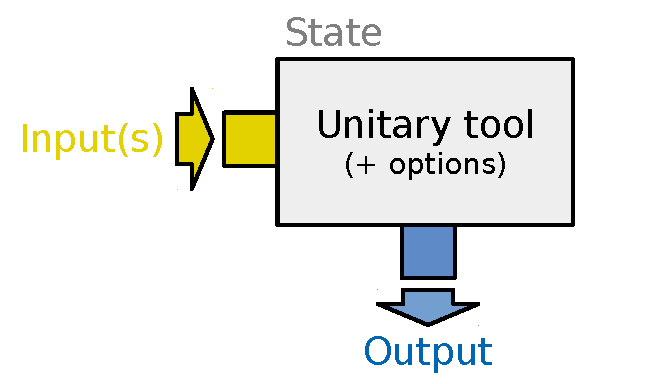
\includegraphics[width=0.4\textwidth]{schemas/PyTelTools_tool.pdf}

  \begin{columns}[onlytextwidth]
  \begin{column}{0.5\textwidth}
\begin{itemize}
    \item<1-> Each \textbf{unitary tool}:
      \begin{itemize}
      \item State {\tiny (Not configured, Ready, Sucess)}
      \item Options (configure)
      \item Input(s)/Output
      \end{itemize}
    \item<2-> \textbf{Combine them} in a \textbf{Directed Acyclic Graph} (DAG)
      \begin{itemize}
        \item data-type correctness
        \item junction
        \item data flows downward
        \item filters
        \item commutativity is sometimes possible (flexibility)
        \item<3> reproductability (project file)
        \item<3> reentrancy (intermediate files)
      \end{itemize}
\end{itemize}
  \end{column}
  \begin{column}{0.48\textwidth}
    \includegraphics<1>[width=0.8\textwidth]{schemas/PyTelTools_tool.pdf}\vspace{1cm}
    \includegraphics<1>[width=0.98\textwidth]{schemas/schema0.png}
    \includegraphics<2>[width=0.98\textwidth]{schemas/schema1bis.png}
    \includegraphics<3>[width=0.98\textwidth]{schemas/schema2.png}
  \end{column}
\end{columns}

\end{frame}


\subsection{Mono view}

\begin{frame}{Demo on Mono view}
  \centering
  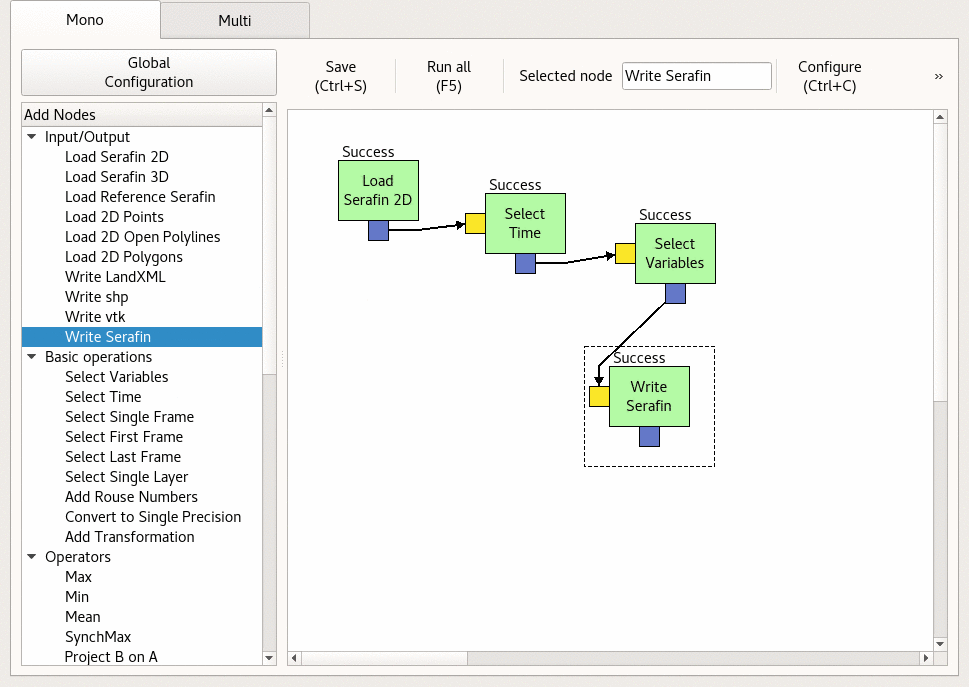
\includegraphics[height=7cm]{animation/mono_demo-430}
\end{frame}


\subsection{Multi view}

\begin{frame}{Repeat over multiple simulation}
  \begin{itemize}
    \item Prerequisites
    \begin{itemize}
      \item the graph is already configured
      \item input data are mostly identical and follows a naming convention
    \end{itemize}
    \item repeat over this serie of simulations
    \item parallelize on multiple CPU
    \item monitoring: status table, log events
  \end{itemize}
\end{frame}

\begin{frame}{Demo on Multi view}
  \centering
  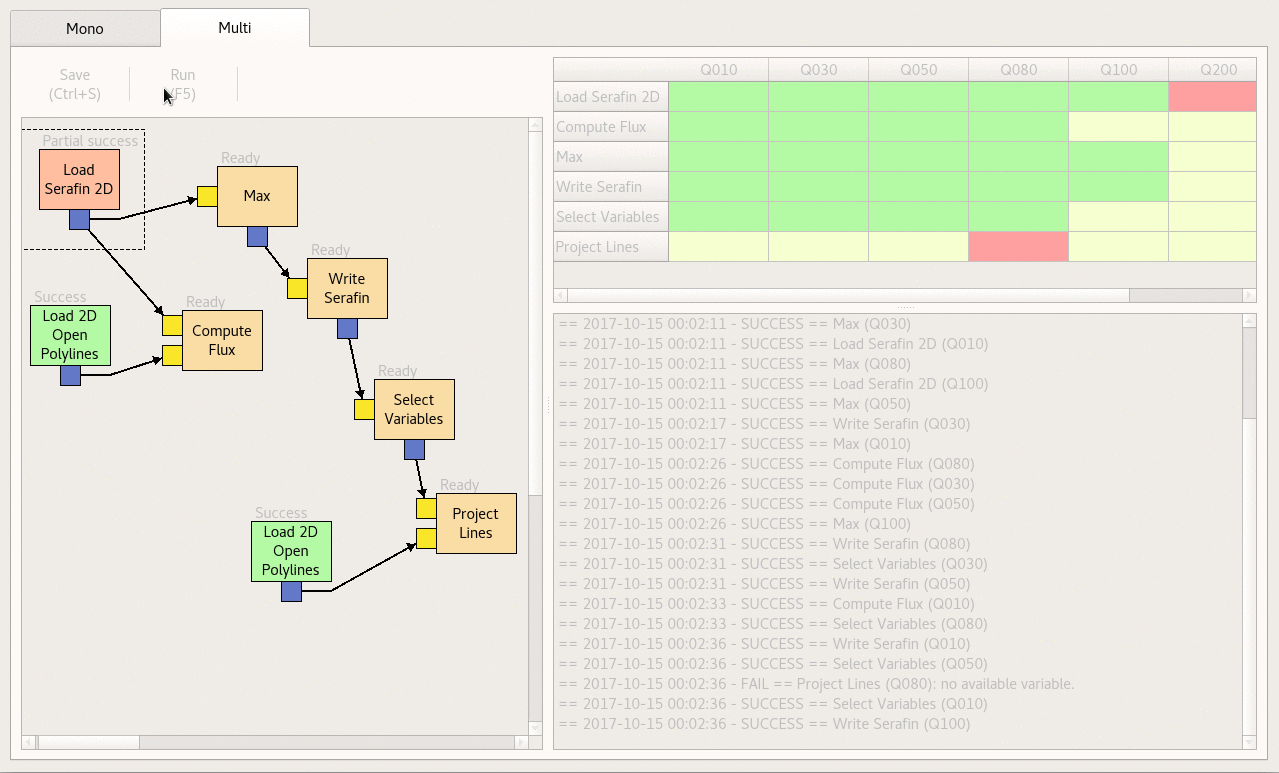
\includegraphics[height=7cm]{animation/multi_demo-181}
\end{frame}



\section{Conclusion}

\begin{frame}{Conclusion}
  \begin{itemize}
    \item Python scripts developped from scratch for Telemac post-processing
    \item accessible through a GUI
    \item open-source, modest contribution
    \item different levels of automation (workflow)
    \item Some \textbf{improvements}:
      \begin{itemize}
        \item compare to measurements, implementation, ...
        \item Unify more Mono and Multi implementation
      \end{itemize}
    \item Coming \textbf{new features} depends on needs (mostly new plots)
  \end{itemize}
\end{frame}

\section*{The End...}

\begin{frame}

\begin{center}
  {\huge Thank you}
  \vspace{1cm}
  \inputminted[fontsize=\Large,xleftmargin=0.4cm]{python}{ending.py}
\end{center}

\end{frame}

\section*{References}
\nocite{internship_report}\nocite{def_math}\nocite{equations}

\begin{frame} % [allowframebreaks] %in case more than 1 slide needed
  {References}
  %\footnotesize
  {\small
  \bibliographystyle{plainurl} % apalike
  \bibliography{reference}
  }
\end{frame}


\end{document}
